\chapter{Planificación y estimación de costes.}

\section{Temporización}

\begin{table}[!h]
\centering
\begin{tabular}{|l|l|l|}
\hline
Nombre & Fecha de inicio & Fecha de fin \\ \hline
Planteamiento de la propuesta & 3/2/20 & 28/2/20 \\ \hline
Investigación sobre SDN & 2/3/20 & 29/5/20 \\ \hline
Desarrollo de la memoria & 16/6/20 & 8/9/20 \\ \hline
Diseño de la red & 1/6/20 & 8/6/20 \\ \hline
Pruebas con Ryu & 22/6/20 & 9/7/20 \\ \hline
Implementación del controlador & 20/7/20 & 2/9/20 \\ \hline
Evaluación de la red & 3/9/20 & 7/9/20 \\ \hline
\end{tabular}
\label{tab:temporizacion}
\caption{Temporización del proyecto}
\end{table}

Este proyecto se ha planificado siguiendo la temporización que se detalla en la tabla \ref{tab:temporizacion}, contando con periodos vacacionales.

Reflejado en un diagrama de Gantt la temporización ha sido la siguiente:

\begin{figure}[!h]
    \centering
    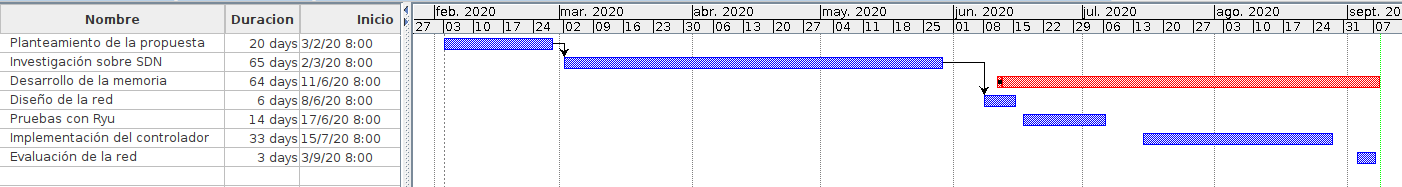
\includegraphics[width=1.2\textwidth]{imagenes/figuras/temporizacion.png}
    \caption{Diagrama de Gantt del proyecto}
    \label{fig:temporizacion}
\end{figure}

\section{Presupuesto}

Si tuviéramos que implementar este proyecto en un entorno físico tendríamos una serie de gastos que vamos a reflejar a continuación. En este presupuesto no se incluyen los nodos cliente de la red ni el cableado, solo lo necesario para que la red definida por software funcione correctamente. Vamos a optar por switches de la marca Mikrotik por su compatibilidad con OpenFlow y su bajo precio. Para ejecutar el controlador Ryu y el servidor DHCP vamos a utilizar un sistema basado en una Raspberry Pi 4, que ofrece suficiente capacidad de computación para la tarea a desempeñar.

El presupuesto queda de la siguiente manera:

\begin{figure}[!h]
\centering
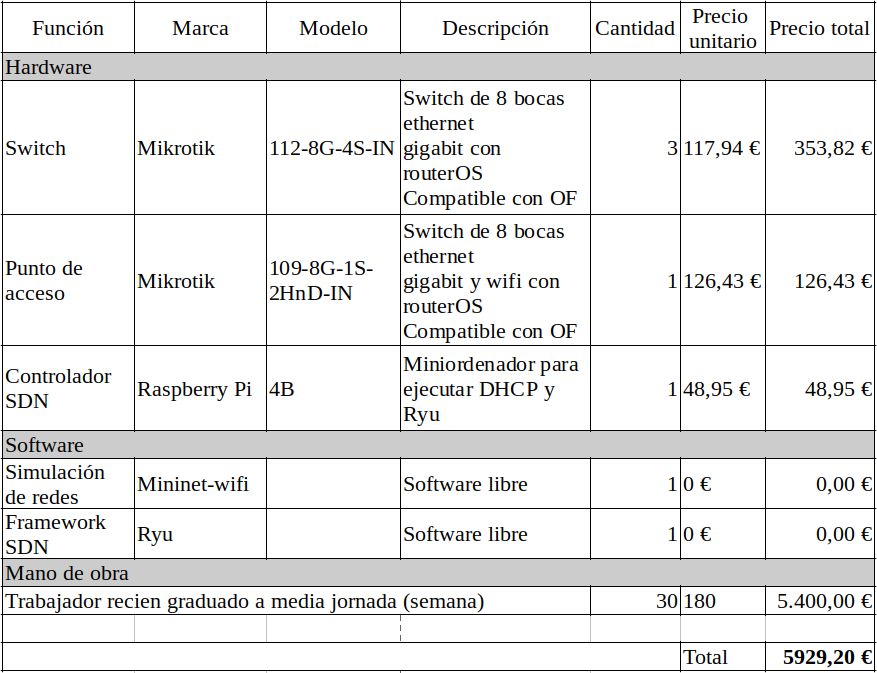
\includegraphics[width=\textwidth]{imagenes/figuras/presupuesto.png}
\label{tab:presupuesto}
\caption{Presupuesto del proyecto}
\end{figure}

La diferencia con un presupuesto con una red tradicional (no SDN) es la Raspberry Pi. Si comparamos su precio con el ahorro que supone la configuración automática de nuevos nodos en materia de gastos de personal y de tiempo de mantenimiento de la red podemos afirmar que merece la pena estructurar la red como una Red Definida por Software. El precio de la mano de obra se ha calculado como 30 semanas de trabajo a media jornada teniendo en cuenta los salarios medios de los ingenieros informáticos recién graduados \cite{Cuantoco58:online}